% !TEX program = pdflatex
\documentclass[11pt,a4paper]{article}

\usepackage[margin=2.5cm]{geometry}
\usepackage{amsmath,amssymb,bm}
\usepackage{graphicx}
\usepackage{booktabs}
\usepackage{siunitx}
\usepackage{microtype}
\usepackage{caption}
\usepackage{subcaption}
\usepackage{float}
\usepackage[section]{placeins}
\usepackage{enumitem}
\usepackage{indentfirst}
\usepackage[numbers,sort&compress]{natbib}
\usepackage[hidelinks]{hyperref}
\usepackage{lmodern}

\graphicspath{{../reproducible/figures/}{./}}
\setlength{\parindent}{1.5em}
\setlength{\parskip}{0.18em}
\captionsetup{font=small,labelfont=bf}
\sisetup{round-mode=places,round-precision=4}
\raggedbottom

\title{\textbf{\Large Numerical Option Pricing and Dynamic Delta Hedging}\\[0.4em]
\large Convergence, Convexity Exposure, and Transaction Costs}
\author{Zhengli Ji\\
Department of Applied Mathematics, Xi'an Jiaotong-Liverpool University}
\date{October 2026}

\begin{document}
% Auto-generated by python -m option_hedging reproduce. Do not edit manually.
\newcommand{\BSValue}{9.413403}
\newcommand{\MCSlope}{-0.526}
\newcommand{\MCSE}{0.016}
\newcommand{\MCCILow}{-0.577}
\newcommand{\MCCIHigh}{-0.476}
\newcommand{\MCRSquared}{0.997}
\newcommand{\CRRSlope}{-0.999}
\newcommand{\MonthlyRMSE}{1.9177}
\newcommand{\DailyRMSE}{0.4317}
\newcommand{\HedgeRMSEDropPct}{77.5}
\newcommand{\WeeklyGammaPearson}{0.903}
\newcommand{\WeeklyGammaSpearman}{0.950}
\newcommand{\WeeklyGammaCILow}{0.709}
\newcommand{\WeeklyGammaCIHigh}{0.990}
\newcommand{\WeeklyPathPearson}{0.574}
\newcommand{\WeeklyPathSpearman}{0.715}
\newcommand{\BestTwentyFiveFrequency}{Weekly}
\newcommand{\BestTwentyFiveRMSE}{1.1430}
\newcommand{\DailyTwentyFiveRMSE}{1.4173}
\newcommand{\DailyTenMeanError}{-0.503}
\newcommand{\BaselineDelta}{0.5987}
\newcommand{\BaselineGamma}{0.0193}
\newcommand{\BaselineVega}{38.67}
\newcommand{\BaselineTheta}{-5.38}
\newcommand{\OTMPriceVolTen}{0.0896}
\newcommand{\OTMPriceVolFifty}{10.2095}
\newcommand{\OTMDeltaVolTen}{0.030}
\newcommand{\OTMDeltaVolFifty}{0.446}
\newcommand{\ITMDeltaVolTen}{0.985}
\newcommand{\ITMDeltaVolFifty}{0.750}
\newcommand{\GammaTTwo}{0.0133}
\newcommand{\GammaTOne}{0.0193}
\newcommand{\GammaTQuarter}{0.0396}
\newcommand{\GammaTTenth}{0.0629}
\newcommand{\ThetaTTenth}{-14.09}


\maketitle

\begin{abstract}
This study investigates numerical option pricing and discrete hedging within the Black--Scholes framework, with particular emphasis on convergence behaviour, risk sensitivities, hedging error, and transaction-cost effects. A European call option is valued analytically and approximated using Monte Carlo simulation and the Cox--Ross--Rubinstein (CRR) binomial model. Monte Carlo experiments reproduce the expected $O(N^{-1/2})$ convergence rate, while the tested even-step CRR sequence exhibits an approximately $O(N^{-1})$ pricing-error pattern together with a clear odd--even lattice oscillation. Sensitivity analysis shows that option value and the principal Greeks depend strongly on the underlying price, volatility, and time to maturity, with Gamma becoming highly concentrated near the strike for short-dated at-the-money options. Discrete delta-hedging simulations demonstrate that increasing the rebalancing frequency substantially reduces replication error in a frictionless market. Across different moneyness, maturity, and hedge-frequency settings, larger integrated Gamma exposure is consistently associated with higher terminal hedging RMSE. A second-order Taylor--It\^o approximation provides the theoretical motivation for this exposure measure, but the empirical relationship is interpreted as association rather than causality. Finally, proportional transaction costs create an accuracy--cost trade-off: at sufficiently high tested cost levels, the highest-frequency strategy no longer minimises net hedging RMSE among the candidate schedules. The study therefore connects analytical pricing, numerical convergence, convexity exposure, discrete replication, and trading frictions within a unified computational framework.
\end{abstract}

\noindent\textbf{Keywords:} Black--Scholes; Monte Carlo; CRR binomial tree; delta hedging; Gamma exposure; transaction costs; numerical finance

\section{Introduction}

Option pricing and dynamic hedging are fundamental problems in quantitative finance because derivative values depend not only on the current state of the underlying asset but also on the way uncertainty evolves over time. The Black--Scholes--Merton framework provides an analytical foundation for this problem, showing that a European option can be valued through no-arbitrage arguments and dynamic replication under idealised assumptions \citep{blackscholes1973,merton1973}. Despite its assumptions of constant volatility, continuous trading, and frictionless markets, it remains a useful benchmark for studying derivative valuation and hedge implementation.

Numerical methods are essential when closed-form solutions are unavailable or inconvenient. Monte Carlo simulation estimates discounted risk-neutral expectations and is flexible for high-dimensional and path-dependent problems \citep{boyle1977,boylebroadieglasserman1997,glasserman2004}. The Cox--Ross--Rubinstein (CRR) model provides a different approximation through a recombining price lattice and risk-neutral transition probabilities \citep{coxrossrubinstein1979}. Both methods converge toward the Black--Scholes value for the European call considered here, but their numerical errors arise from different mechanisms: Monte Carlo error is stochastic, whereas lattice error is deterministic and can oscillate with the step count.

Pricing accuracy alone does not characterise the practical difficulty of managing an option position. Black--Scholes replication assumes that the hedge ratio can be adjusted continuously. Real portfolios are rebalanced only at discrete times, so Delta becomes temporarily outdated between hedge dates. This creates replication error even when the underlying follows the assumed diffusion. The problem is particularly relevant in regions of high Gamma, where Delta changes rapidly with the underlying price \citep{boyleemanuel1980,bertsimaskoganlo2000,gobettemam2001}.

Trading frictions add a second implementation problem. More frequent rebalancing reduces the time for which the hedge is stale, but it also increases turnover and transaction costs. Research on discrete replication with proportional costs shows that continuous frictionless hedging cannot be transferred directly to a costly market \citep{leland1985,boylevorst1992,davispanaszariphopoulou1993,toft1996}. The resulting trade-off motivates a joint analysis of discretisation error and implementation cost.

This study addresses four research questions:
\begin{enumerate}[label=\textbf{RQ\arabic*:},leftmargin=2.2cm]
    \item How accurately do Monte Carlo simulation and the CRR binomial model approximate the Black--Scholes value of a European call option, and how do their convergence patterns differ?
    \item How do the underlying asset price, volatility, and time to maturity affect the option value and its principal Greeks?
    \item How does discrete delta-rebalancing frequency affect hedging error, and how is terminal replication risk associated with cumulative Gamma exposure?
    \item How do proportional transaction costs affect the relationship between hedge frequency and hedging performance?
\end{enumerate}

The contribution is computational and integrative rather than a claim to a new pricing model. The analysis uses a common specification to connect pricing convergence, local risk sensitivity, discrete replication, a theoretically motivated integrated Gamma-exposure measure, and proportional transaction costs. Figure~\ref{fig:methodology} summarises this progression.

\begin{figure}[htbp]
    \centering
    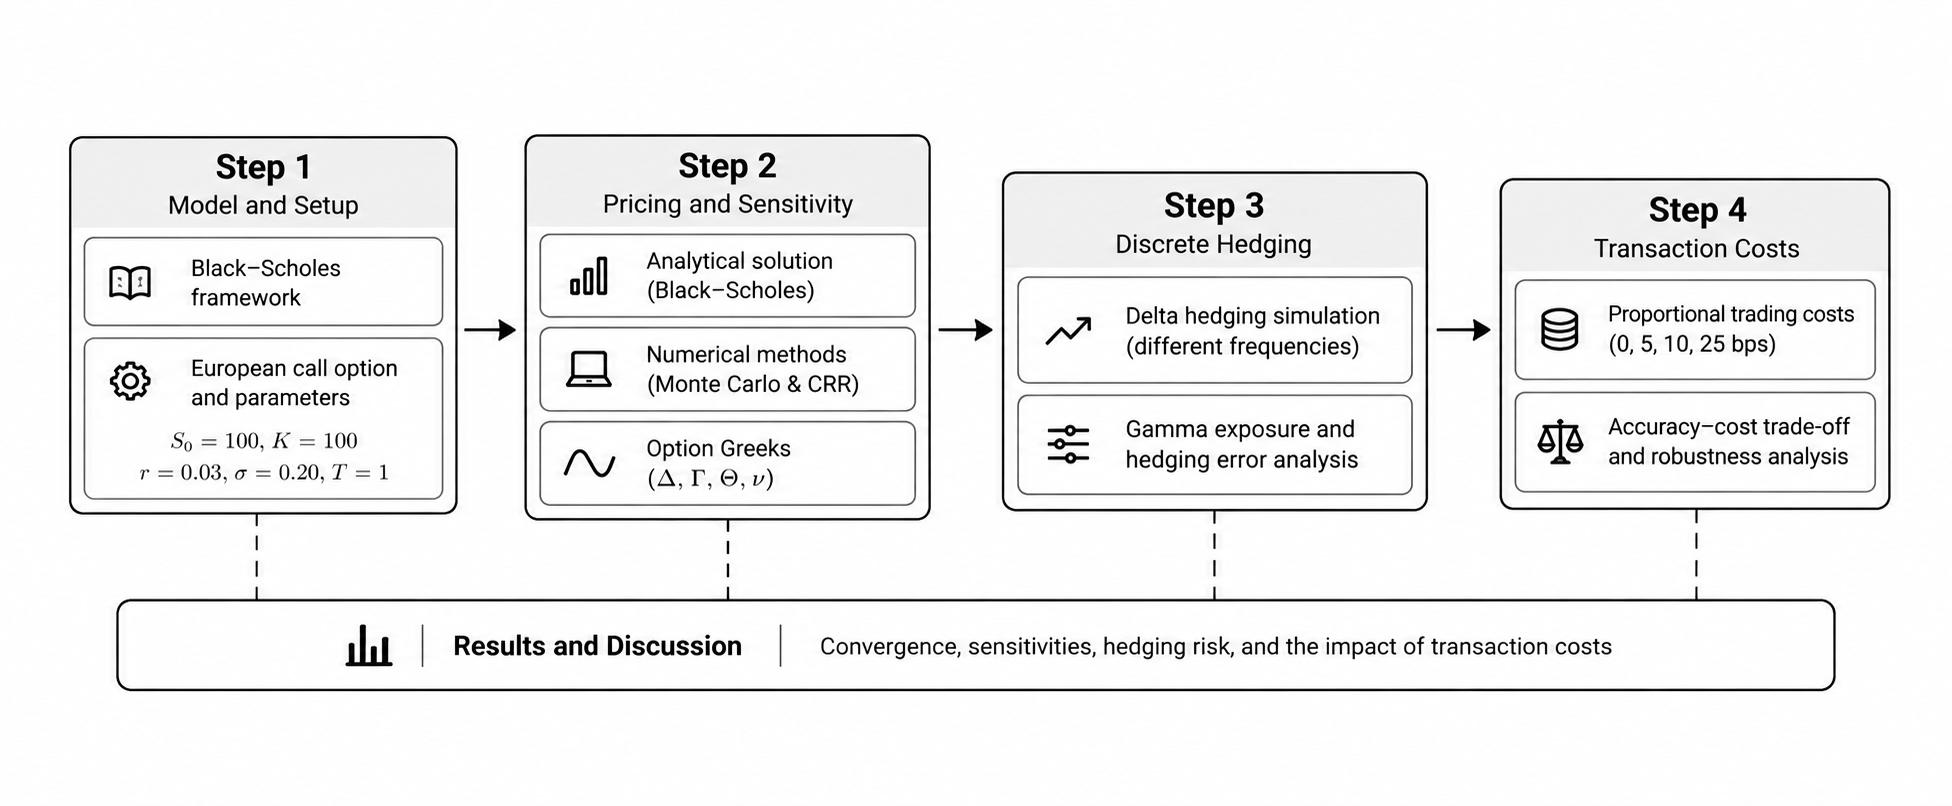
\includegraphics[width=1\textwidth]{methodology_framework_horizontal.png}
    \caption{Research framework and methodological workflow.}
    \label{fig:methodology}
\end{figure}
\section{Literature Review}

\subsection{Analytical Pricing and Numerical Valuation}

Modern option-pricing theory is founded on no-arbitrage and dynamic replication. \citet{blackscholes1973} derive the value of a European option from a continuously adjusted replicating portfolio, while \citet{merton1973} provides a broader continuous-time foundation for rational option pricing. These contributions establish the analytical benchmark used throughout this study.

Monte Carlo valuation was introduced to option pricing by \citet{boyle1977}, who showed that derivative values can be estimated by simulating the risk-neutral dynamics of the underlying and averaging discounted payoffs. Subsequent work emphasises both the flexibility and the slow square-root convergence of standard simulation. \citet{boylebroadieglasserman1997} review variance-reduction, quasi-Monte Carlo, sensitivity estimation, and simulation-based valuation, while \citet{glasserman2004} provides a systematic treatment of Monte Carlo methods in financial engineering. Applications such as the control-variate approach of \citet{kemnavorst1990} illustrate how analytical structure can improve simulation efficiency. The present study does not add a variance-reduction scheme; these contributions instead provide context for interpreting the empirical $O(N^{-1/2})$ rate of the standard estimator.

The CRR model discretises the diffusion into a recombining binomial tree \citep{coxrossrubinstein1979}. Its convergence can be non-monotonic because terminal nodes change their alignment with the strike as the number of steps changes. \citet{leisenreimer1996} document distorted and oscillatory convergence patterns and show that tree design can improve both smoothness and speed. \citet{hestonzhou2000} relate discrete-time convergence to payoff smoothness, an important issue for the kinked European-call payoff. \citet{dienerdiener2004} derive asymptotic results for oscillations in European-call tree prices, while \citet{changpalmer2007} examine constructions designed to produce smoother convergence. This literature motivates separating odd and even CRR subsequences rather than fitting one rate across an oscillating sequence.

\subsection{Discrete Hedging, Gamma, and Replication Error}

Continuous-time replication is a limiting idealisation. \citet{boyleemanuel1980} analyse discretely adjusted option hedges and show that the distribution of hedged-portfolio returns can be strongly non-normal. \citet{bertsimaskoganlo2000} characterise the asymptotic distribution of replication errors and show that root-mean-squared tracking error is of order $N^{-1/2}$ under their setting. \citet{gobettemam2001} further show that the rate of discrete-time hedging error depends on payoff regularity.

Gamma provides the local link between movements in the underlying and changes in Delta. A second-order expansion implies that, after first-order Delta exposure is offset, local residual error is governed in part by the convexity term involving $\Gamma(\Delta S)^2$. This does not mean that Gamma alone determines terminal error: the realised path, the timing of moves, higher-order terms, and the rebalancing grid also matter. The literature on discrete hedging therefore supports a theoretically motivated association between cumulative convexity exposure and replication risk, rather than a causal one-variable explanation.

\subsection{Transaction Costs and Hedge Frequency}

Once proportional transaction costs are introduced, perfect continuous replication is no longer feasible. \citet{leland1985} modifies the replication argument to account for costs generated by frequent rebalancing. In discrete time, \citet{boylevorst1992} extend the binomial replication framework to proportional costs, and \citet{davispanaszariphopoulou1993} formulate European option pricing with costs as a stochastic control problem in which perfect replication is replaced by utility-based valuation.

The trade-off between hedge risk and trading cost is examined directly by \citet{toft1996}, who derives cost and risk characteristics for discretely rebalanced strategies. \citet{grannanswindle1996} consider hedging rules designed to reduce expected replication error subject to costs, including strategies with non-uniform hedge intervals. \citet{whalleywilmott1997} use asymptotic analysis to derive an optimal-hedging approximation whose no-transaction structure depends explicitly on option Gamma. Collectively, these studies establish that an empirically preferred hedge frequency must be interpreted as conditional on the assumed cost process, contract, and evaluation criterion. The present experiment therefore reports the best schedule only within the tested frequency and cost grid.

The literature supplies mature results for each individual component of the study. The purpose here is to integrate them in a transparent experiment: analytical and numerical pricing are benchmarked first; Greek behaviour identifies high-convexity regions; discrete hedging then quantifies replication risk; and transaction costs finally test whether the frictionless frequency ranking survives implementation frictions.

\section{Mathematical Framework}

\subsection{Risk-Neutral Stock Dynamics}

Under the physical measure, the stock price follows geometric Brownian motion,
\begin{equation}
    dS_t=\mu S_t\,dt+\sigma S_t\,dW_t,
\end{equation}
where $\mu$ is the expected return, $\sigma>0$ is volatility, and $W_t$ is Brownian motion. Under the risk-neutral measure $Q$, the drift is replaced by the continuously compounded risk-free rate $r$:
\begin{equation}
    dS_t=rS_t\,dt+\sigma S_t\,dW_t^Q.
\end{equation}
The exact terminal distribution is
\begin{equation}
    S_T=S_0\exp\left[\left(r-\frac{1}{2}\sigma^2\right)T+\sigma\sqrt{T}Z\right],
    \qquad Z\sim N(0,1).
\end{equation}

\subsection{Black--Scholes Benchmark}

For a derivative value $V(S,t)$, It\^o's lemma and a locally delta-neutral portfolio lead to the Black--Scholes partial differential equation
\begin{equation}
    \frac{\partial V}{\partial t}
    +\frac{1}{2}\sigma^2S^2\frac{\partial^2V}{\partial S^2}
    +rS\frac{\partial V}{\partial S}-rV=0.
\end{equation}
For a non-dividend-paying European call with remaining maturity $\tau=T-t$,
\begin{equation}
    C(S,t)=SN(d_1)-Ke^{-r\tau}N(d_2),
\end{equation}
where
\begin{align}
    d_1&=\frac{\ln(S/K)+(r+\tfrac{1}{2}\sigma^2)\tau}{\sigma\sqrt{\tau}},\\
    d_2&=d_1-\sigma\sqrt{\tau}.
\end{align}
Table~\ref{tab:baseline} reports the baseline specification.

\begin{table}[H]
\centering
\caption{Baseline Black--Scholes parameters.}
\label{tab:baseline}
\begin{tabular}{lc}
\toprule
Parameter & Value \\
\midrule
Initial stock price $S_0$ & 100 \\
Strike price $K$ & 100 \\
Risk-free rate $r$ & 3\% \\
Volatility $\sigma$ & 20\% \\
Time to maturity $T$ & 1 year \\
Dividend yield & 0 \\
Option type & European call \\
Black--Scholes benchmark $C_{BS}$ & 9.4134 \\
\bottomrule
\end{tabular}
\end{table}

\subsection{Monte Carlo and CRR Valuation}

Risk-neutral valuation gives
\begin{equation}
    C_0=e^{-rT}\mathbb{E}^{Q}[(S_T-K)^+].
\end{equation}
With $N$ independently simulated terminal prices, the Monte Carlo estimator is
\begin{equation}
    \widehat C_N=e^{-rT}\frac{1}{N}\sum_{j=1}^{N}(S_T^{(j)}-K)^+.
\end{equation}
For finite payoff variance, $\operatorname{SE}(\widehat C_N)=O(N^{-1/2})$.

For a CRR tree with $N$ time steps and $\Delta t=T/N$,
\begin{equation}
    u=e^{\sigma\sqrt{\Delta t}},\qquad d=e^{-\sigma\sqrt{\Delta t}},
\end{equation}
and the risk-neutral up probability is
\begin{equation}
    p=\frac{e^{r\Delta t}-d}{u-d}.
\end{equation}
Terminal payoffs are discounted recursively:
\begin{equation}
    V_t=e^{-r\Delta t}\left[pV_u+(1-p)V_d\right].
\end{equation}

\subsection{Greeks and Discrete Delta Hedging}

For a European call,
\begin{equation}
    \Delta=\frac{\partial C}{\partial S}=N(d_1),
\end{equation}
and
\begin{equation}
    \Gamma=\frac{\partial^2C}{\partial S^2}
    =\frac{\phi(d_1)}{S\sigma\sqrt{\tau}}.
\end{equation}
The other principal sensitivities used in the parameter analysis are
\begin{equation}
    \text{Vega}=S\phi(d_1)\sqrt{\tau}
\end{equation}
and
\begin{equation}
    \Theta=-\frac{S\phi(d_1)\sigma}{2\sqrt{\tau}}
    -rKe^{-r\tau}N(d_2).
\end{equation}

At hedge date $t_i$, the replicating portfolio is
\begin{equation}
    V_{t_i}=\Delta_{t_i}S_{t_i}+B_{t_i},
\end{equation}
where $B_{t_i}$ is the cash position. With a fixed hedge interval $\Delta t$, the cash account evolves according to
\begin{equation}
    B_{t_{i+1}}=B_{t_i}e^{r\Delta t}
    -(\Delta_{t_{i+1}}-\Delta_{t_i})S_{t_{i+1}}.
\end{equation}
The terminal hedging error is
\begin{equation}
    E_T=V_T-(S_T-K)^+.
\end{equation}

\subsection{Second-Order Motivation for Integrated Gamma Exposure}
\label{sec:gamma_motivation}

Consider one hedge interval $[t_i,t_{i+1}]$. A second-order Taylor--It\^o approximation of the option-value change is
\begin{equation}
\Delta C_i
\approx
\Theta_{t_i}\Delta t
+\Delta_{t_i}\Delta S_i
+\frac{1}{2}\Gamma_{t_i}(\Delta S_i)^2,
\label{eq:taylor}
\end{equation}
where $\Delta S_i=S_{t_{i+1}}-S_{t_i}$. The stock position removes the first-order term $\Delta_{t_i}\Delta S_i$. Using the Black--Scholes PDE to combine Theta, financing, and the conditional diffusion variance gives the leading local residual in the approximate form
\begin{equation}
\varepsilon_i
\approx
\frac{1}{2}\Gamma_{t_i}
\left[(\Delta S_i)^2-\sigma^2S_{t_i}^2\Delta t\right].
\label{eq:local_residual}
\end{equation}
Under the model, the bracketed term is centred to first order, but its realised magnitude is random. Equation~\eqref{eq:local_residual} shows why large $|\Gamma|$, a large underlying level, high volatility, and a longer interval between hedge updates can amplify the scale of discrete replication error. This interpretation is consistent with the discrete-hedging literature \citep{boyleemanuel1980,bertsimaskoganlo2000,gobettemam2001}.

Motivated by the scale of the second-order term, the study defines pathwise integrated Gamma exposure as
\begin{equation}
    G=\sum_i\frac{1}{2}|\Gamma_{t_i}|S_{t_i}^2\sigma^2\Delta t.
\label{eq:gamma_exposure}
\end{equation}
The absolute Gamma makes $G$ a non-negative exposure measure, while $\sigma^2S^2\Delta t$ represents the local variance scale of the stock move. Importantly, $G$ is not an exact signed decomposition of $E_T$. It does not preserve the realised sign of $(\Delta S_i)^2-\sigma^2S_{t_i}^2\Delta t$, and it omits higher-order terms, path timing, and interaction with the rebalancing grid. Because both $G$ and $E_T$ depend on the same realised price path, an empirical correlation between them is interpreted as an association and risk indicator, not as evidence that $G$ independently causes hedging error.

\subsection{Transaction Costs}

If the stock position changes from $\Delta_{t_i}$ to $\Delta_{t_{i+1}}$, proportional transaction costs are
\begin{equation}
    \operatorname{TC}_{t_{i+1}}
    =c\left|\Delta_{t_{i+1}}-\Delta_{t_i}\right|S_{t_{i+1}},
\end{equation}
where $c$ is the cost rate per dollar traded. The cash update becomes
\begin{equation}
    B_{t_{i+1}}=B_{t_i}e^{r\Delta t}
    -(\Delta_{t_{i+1}}-\Delta_{t_i})S_{t_{i+1}}
    -\operatorname{TC}_{t_{i+1}}.
\end{equation}

\section{Methodology}

\subsection{Research Design}

The empirical analysis consists of controlled numerical experiments under a consistent Black--Scholes specification. Unless otherwise stated,
\[
S_0=100,\qquad K=100,\qquad r=3\%,\qquad \sigma=20\%,\qquad T=1.
\]
All computations were implemented in Python using NumPy and SciPy. Fixed random seeds were used for simulation-based experiments.

\subsection{Numerical Pricing Experiments}

For Monte Carlo pricing,
\[
N\in\{10^2,10^3,10^4,10^5,10^6\}
\]
was tested. Each size was repeated 50 times using independent random samples. Across the $R=50$ replications, mean absolute error and root mean squared error were calculated as
\begin{align}
\operatorname{MAE}_N&=\frac{1}{R}\sum_{j=1}^{R}\left|\widehat C_{N,j}-C_{BS}\right|,\\
\operatorname{RMSE}_N&=\sqrt{\frac{1}{R}\sum_{j=1}^{R}(\widehat C_{N,j}-C_{BS})^2}.
\end{align}
The empirical convergence rate was estimated from
\begin{equation}
    \log(\operatorname{MAE}_N)=\alpha+\beta\log N+u_N.
\end{equation}
In addition to the slope, the regression standard error, 95\% confidence interval, and $R^2$ are reported. Because the fit contains only five design points, the interval is treated as a descriptive model-based uncertainty measure rather than a general population claim.

For CRR pricing, the principal lattice sizes were
\[
N\in\{10,25,50,100,250,500,1000\}.
\]
Every integer step count from 10 to 120 was additionally evaluated for oscillation. Because the consecutive sequence alternated, the convergence rate was estimated on the even-step sequence
\[
N\in\{20,40,80,160,320,640,1280\}.
\]

\subsection{Parameter-Sensitivity Analysis}

Three representative moneyness values were used,
\[
S_0=80\ (\text{OTM}),\qquad S_0=100\ (\text{ATM}),\qquad S_0=120\ (\text{ITM}),
\]
with volatility values $\sigma\in\{0.10,0.20,0.50\}$ and maturities $T\in\{0.10,0.25,1.00,2.00\}$ for the tabulated sensitivity grid. Call value, Delta, Gamma, Vega, and Theta were generated analytically for every configured combination. A separate three-dimensional Gamma surface uses $S\in[60,140]$ and $T\in[0.03,2.0]$ at $\sigma=20\%$ to visualise the near-expiry ATM region most relevant to subsequent hedging analysis.

\subsection{Discrete Delta-Hedging Experiment}

A short European call was replicated by a dynamically rebalanced stock-and-cash portfolio. Four annualised hedge frequencies were tested:
\[
12,\qquad52,\qquad126,\qquad252,
\]
corresponding approximately to monthly, weekly, twice-weekly, and daily rebalancing. For each frequency, 5,000 risk-neutral GBM paths were simulated. Performance was summarised by mean error, standard deviation, quantiles, and
\begin{equation}
    \operatorname{RMSE}=\sqrt{\frac{1}{M}\sum_{j=1}^{M}E_{T,j}^2}.
\end{equation}

\subsection{Gamma-Exposure Analysis}

Nine moneyness--maturity scenarios were formed from
\[
S_0\in\{80,100,120\},\qquad T\in\{0.25,0.50,1.00\}.
\]
The nine scenarios were evaluated at each of the four hedge frequencies, using 5,000 simulated paths per scenario. Weekly rebalancing is used as the primary visual comparison, while monthly, twice-weekly, and daily schedules provide robustness checks. Mean integrated Gamma exposure was compared with scenario-level hedging RMSE using Pearson and Spearman correlations. Individual-path association was evaluated by pooling Gamma exposure and absolute terminal hedge error within each hedge-frequency experiment.

Uncertainty for each scenario-level Pearson coefficient was estimated by resampling the corresponding nine scenario pairs with replacement. A percentile bootstrap with 200,000 replications and fixed seed 20260923 produced the reported 95\% confidence intervals. Because only nine deliberately selected scenarios enter each coefficient, the intervals are interpreted as descriptive sensitivity measures rather than population inference.

\subsection{Transaction-Cost Experiment}

Proportional transaction-cost rates of
\[
c\in\{0,0.0005,0.0010,0.0025\}
\]
corresponding to 0, 5, 10, and 25 basis points per dollar traded were applied to the same four hedge frequencies. Following the implementation convention, transaction costs are charged only on internal rebalancing trades: the initial stock purchase used to establish the hedge is not charged, and no terminal stock liquidation is performed or charged. Terminal replication error is therefore evaluated from the remaining stock-and-cash portfolio against the option payoff. Common simulated stock paths were used across cost specifications where appropriate. The objective is to characterise the tested accuracy--cost trade-off, not to identify a universal optimal frequency.

\section{Results}

\subsection{RQ1: Numerical Pricing Accuracy and Convergence}

The Black--Scholes analytical value of the baseline call is
\[
C_{BS}=\BSValue.
\]
Across the five Monte Carlo design points, mean absolute error and RMSE declined as the number of simulated terminal prices increased. The generated pricing table reports representative estimates at $10^4$ and $10^6$ paths.

The log--log regression produced
\[
\widehat\beta=\MCSlope,\qquad \operatorname{SE}(\widehat\beta)=\MCSE,
\]
with a model-based 95\% confidence interval of $[\MCCILow,\MCCIHigh]$ and $R^2=\MCRSquared$. The interval contains the theoretical slope $-1/2$, and the high $R^2$ indicates that the five observed design points closely follow the square-root convergence relationship. Because the fit uses only five aggregate design points, the interval is interpreted descriptively.

The CRR method also converged to the benchmark. Consecutive step counts displayed a pronounced odd--even oscillation, while the specified even-step sequence produced a fitted log--log slope of approximately $\CRRSlope$, consistent with an empirical $O(N^{-1})$ pattern for this European call and CRR construction.

\begin{figure}[H]
    \centering
    \begin{subfigure}[t]{0.48\linewidth}
        \centering
        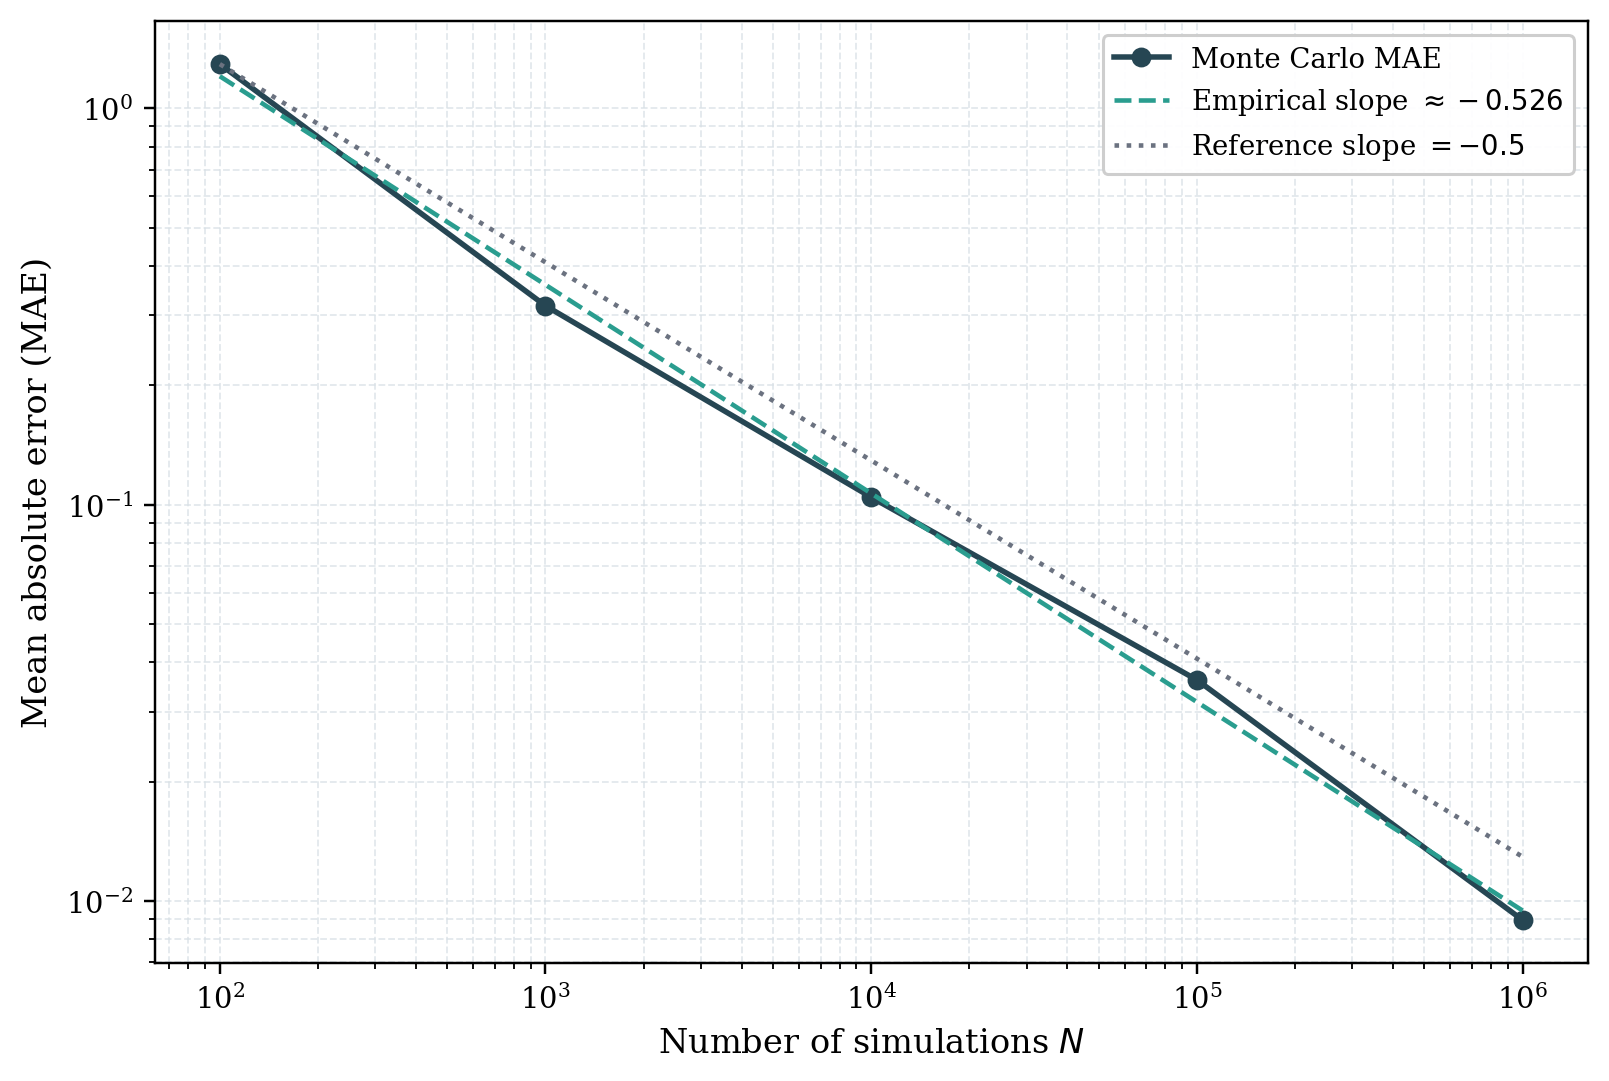
\includegraphics[width=\linewidth]{mc_convergence.png}
        \caption{Monte Carlo error convergence.}
    \end{subfigure}
    \hfill
    \begin{subfigure}[t]{0.48\linewidth}
        \centering
        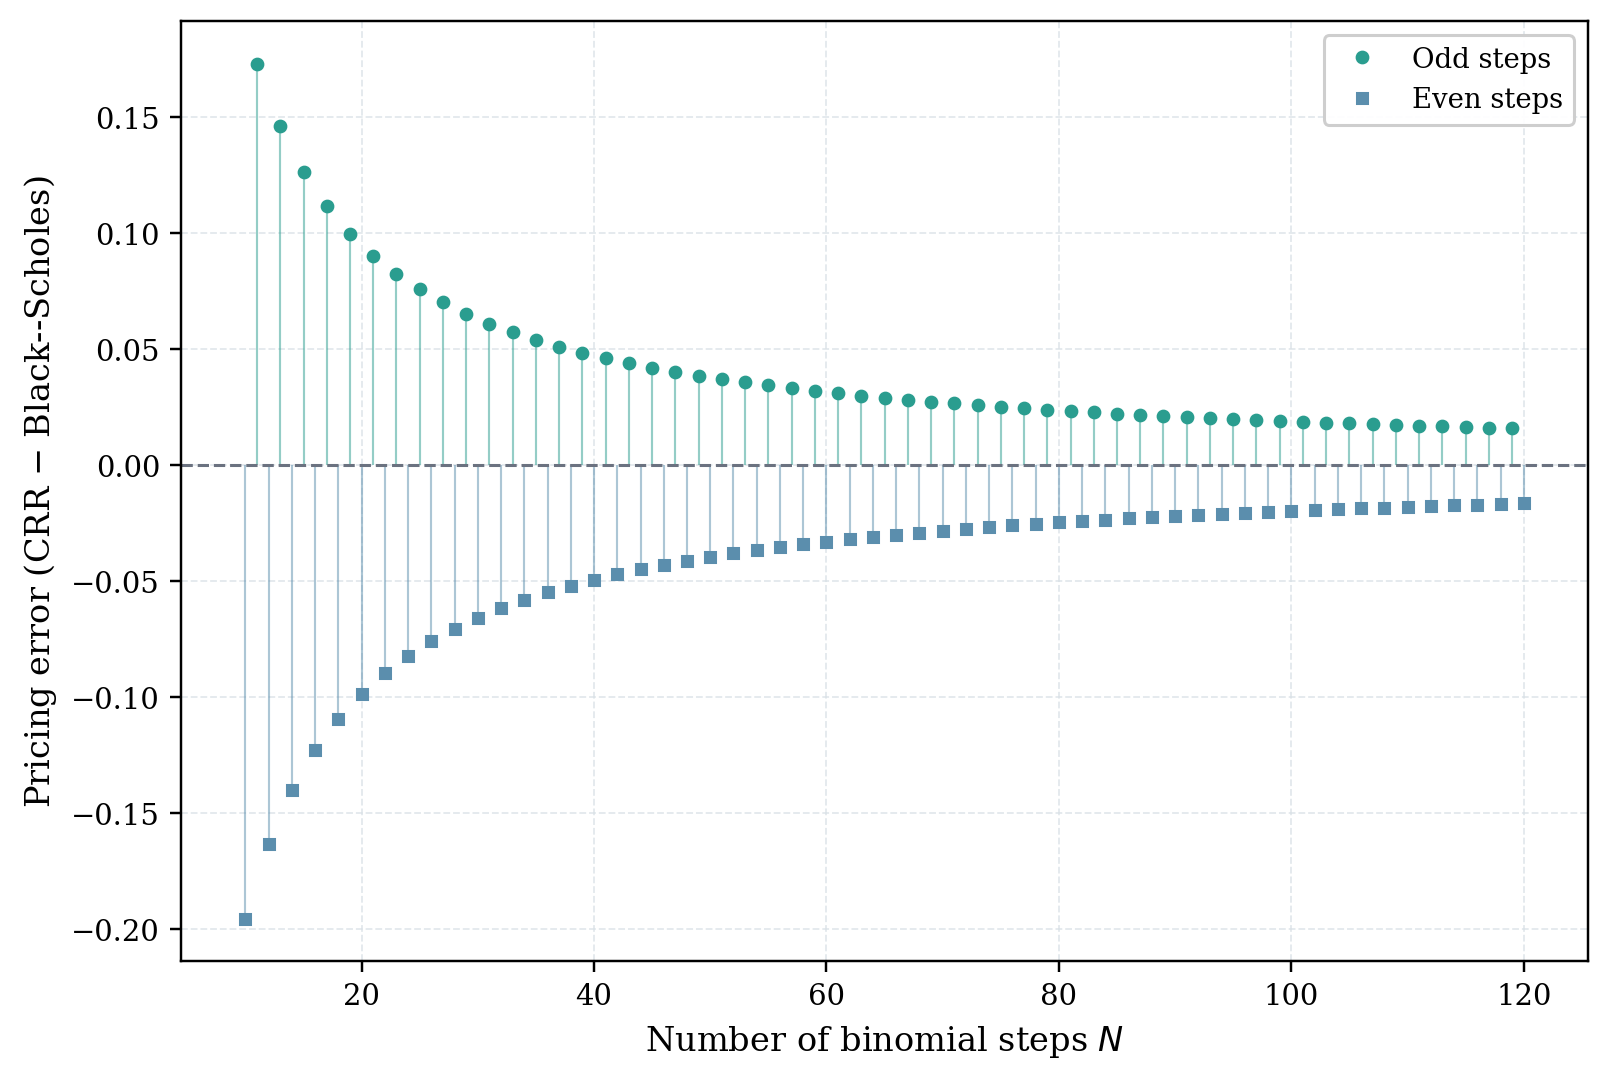
\includegraphics[width=\linewidth]{crr_oscillation.png}
        \caption{CRR odd--even lattice oscillation.}
    \end{subfigure}
    \caption{Numerical convergence relative to the Black--Scholes benchmark.}
    \label{fig:convergence}
\end{figure}

\begin{table}[H]
\centering
\caption{Selected numerical pricing results relative to the Black--Scholes benchmark.}
\label{tab:pricing}
\begin{tabular}{lrrl}
\toprule
Method & Resolution & Price & Error metric \\
\midrule
Black--Scholes & Analytical & 9.4134 & -- \\
Monte Carlo & $10^4$ paths & 9.4659 & MAE 0.1044 \\
Monte Carlo & $10^6$ paths & 9.4094 & MAE 0.0089 \\
CRR & 100 steps & 9.3936 & Abs. error 0.0198 \\
CRR & 1,000 steps & 9.4114 & Abs. error 0.0020 \\
\bottomrule
\end{tabular}
\end{table}


The comparison is deliberately framed in terms of convergence and pricing error rather than wall-clock speed. Runtime depends on hardware, Python build, and implementation details, so it is not treated as a reproducible scientific result in the final study.

\FloatBarrier

\subsection{RQ2: Parameter Sensitivity and Option Greeks}

The call value increased monotonically with the underlying price and volatility over the tested range. At the baseline ATM configuration, $S=K=100$, $\sigma=20\%$, and $T=1$, the Black--Scholes value was \BSValue. For the initially OTM case $S_0=80$, increasing volatility from 10\% to 50\% raised the call value from approximately \OTMPriceVolTen{} to \OTMPriceVolFifty{}.

The effect of volatility on Delta depended on moneyness. For $S_0=80$, Delta increased from approximately \OTMDeltaVolTen{} at $\sigma=10\%$ to \OTMDeltaVolFifty{} at $\sigma=50\%$. For $S_0=120$, Delta declined from approximately \ITMDeltaVolTen{} to \ITMDeltaVolFifty{} over the same volatility range. Volatility therefore changes directional exposure differently across moneyness states.

Gamma exhibited a strong interaction between moneyness and maturity. Figure~\ref{fig:gamma_surface} shows that Gamma becomes increasingly concentrated around the strike as expiry approaches. At $S=100$, Gamma increased from approximately \GammaTTwo{} at $T=2$ years to \GammaTOne{} at $T=1$, \GammaTQuarter{} at $T=0.25$, and \GammaTTenth{} at $T=0.10$.

\begin{figure}[H]
    \centering
    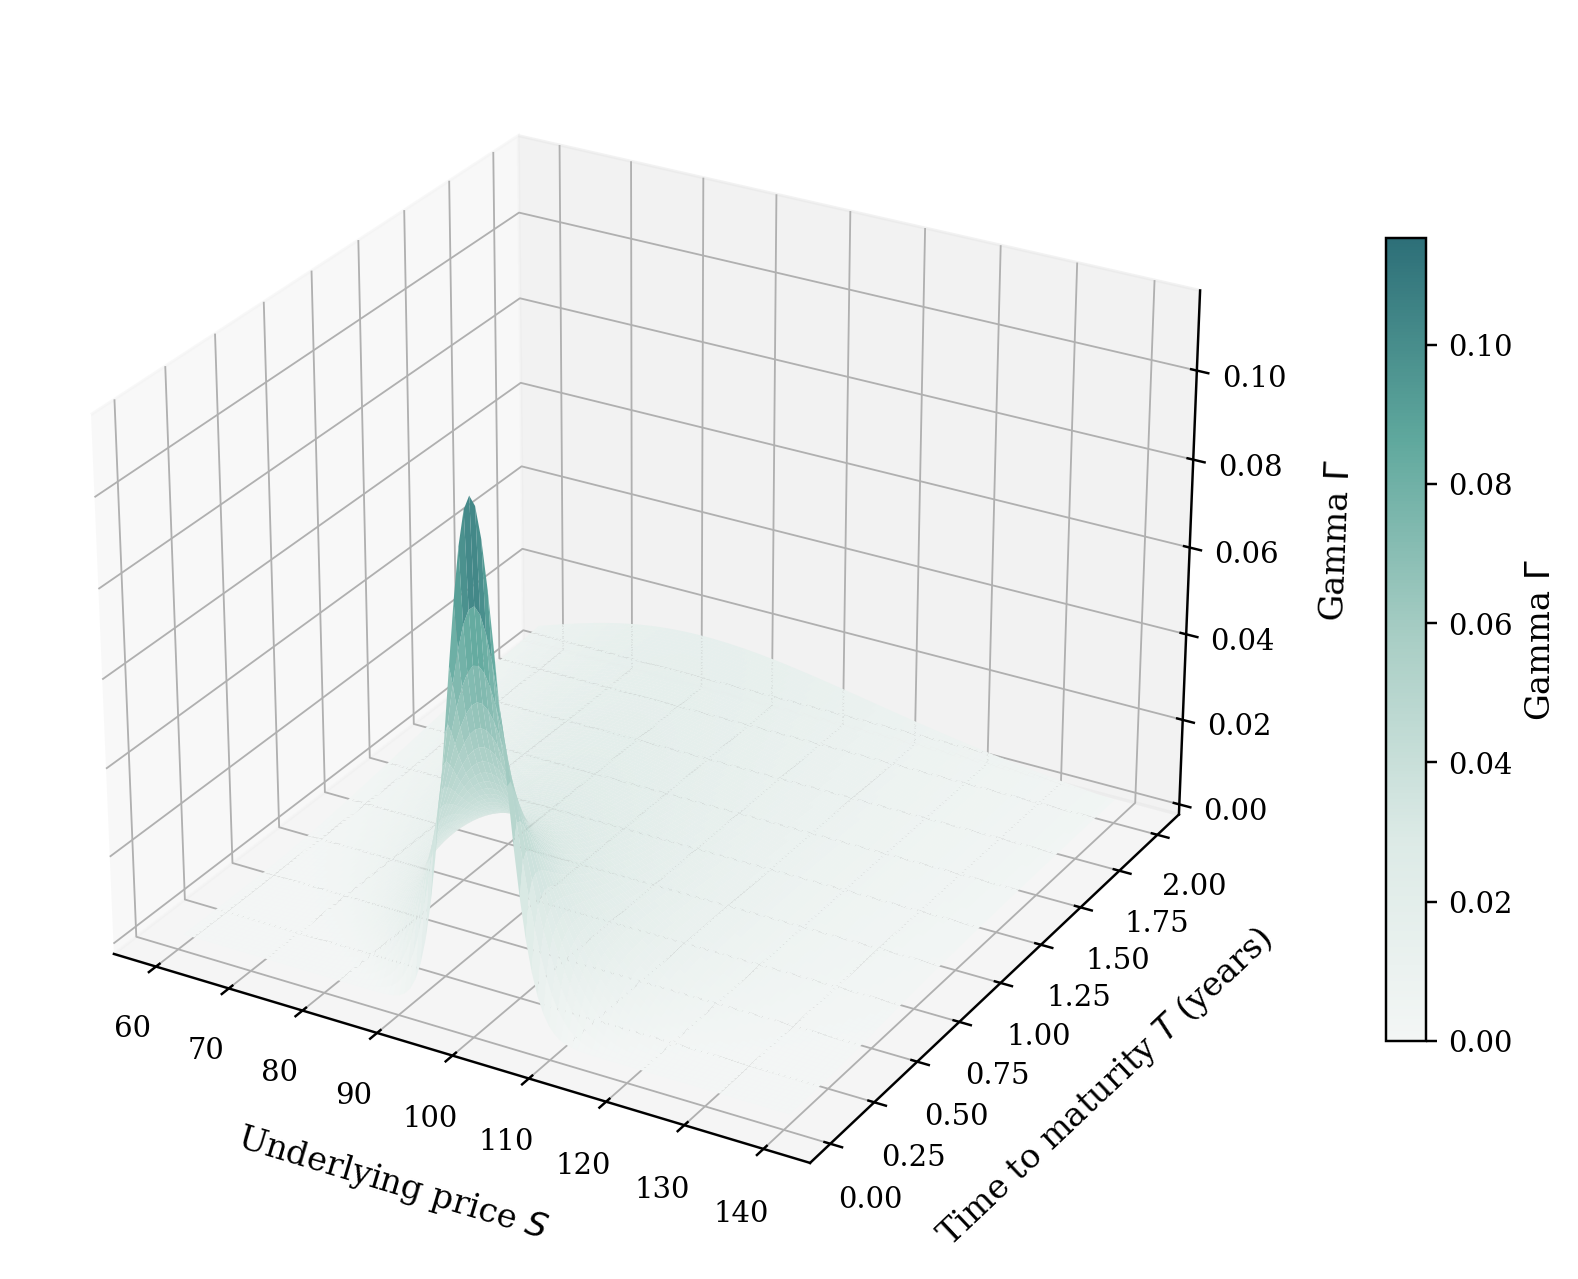
\includegraphics[width=0.80\linewidth]{gamma_surface.png}
    \caption{European-call Gamma across underlying price and time to maturity for $K=100$, $r=3\%$, and $\sigma=20\%$.}
    \label{fig:gamma_surface}
\end{figure}

This near-expiry concentration is much weaker for deep OTM and ITM options, producing a narrow high-Gamma region around the strike. At the baseline ATM point,
\[
\Delta=\BaselineDelta,\qquad \Gamma=\BaselineGamma,\qquad
\text{Vega}=\BaselineVega,\qquad \Theta=\BaselineTheta.
\]
At $S=100$, shortening maturity from one year to 0.10 years changed Theta from approximately $\BaselineTheta$ to $\ThetaTTenth$. Short-dated ATM options are therefore the region in which the hedge ratio changes most rapidly, directly motivating the next experiment.

\FloatBarrier

\subsection{RQ3: Discrete Delta Hedging and Gamma Exposure}

In the frictionless experiment, increasing the rebalancing frequency substantially reduced terminal replication error. Mean terminal errors remained close to zero, while dispersion fell. Moving from 12 to 252 rebalances per year reduced RMSE from \MonthlyRMSE{} to \DailyRMSE{}, a decline of approximately \HedgeRMSEDropPct\% relative to monthly rebalancing.

\begin{table}[H]
\centering
\caption{Frictionless discrete delta-hedging performance.}
\label{tab:hedge}
\begin{tabular}{lrrr}
\toprule
Frequency & Mean error & Std. dev. & RMSE \\
\midrule
Monthly (12) & -0.0024 & 1.9179 & 1.9177 \\
Weekly (52) & 0.0184 & 0.9625 & 0.9626 \\
Approx. twice-weekly (126) & -0.0162 & 0.6176 & 0.6178 \\
Daily (252) & 0.0021 & 0.4318 & 0.4317 \\
\bottomrule
\end{tabular}
\end{table}


\begin{figure}[H]
    \centering
    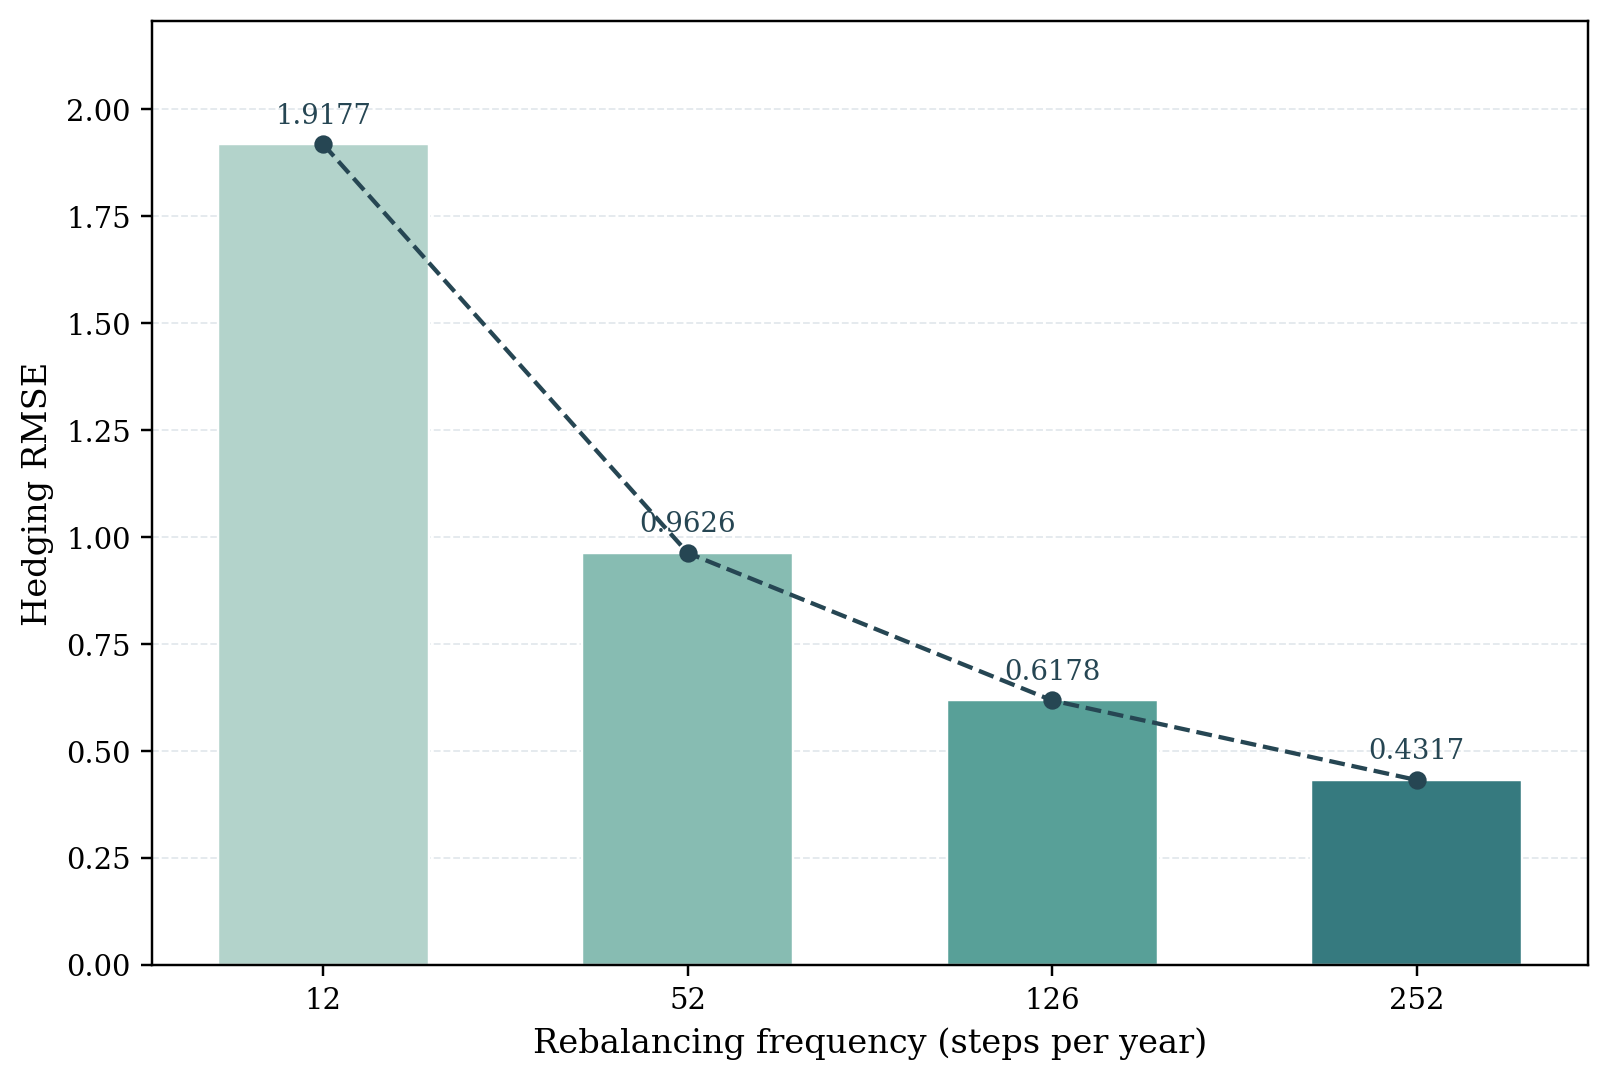
\includegraphics[width=0.55\linewidth]{hedging_rmse.png}
    \caption{Frictionless hedging RMSE across rebalancing frequencies.}
    \label{fig:hedging_rmse}
\end{figure}

The Gamma-exposure experiment provides a complementary cross-scenario result. Under weekly rebalancing, scenarios with greater mean integrated Gamma exposure generally exhibited larger hedging RMSE. The scenario-level Pearson correlation was
\[
\rho=\WeeklyGammaPearson,
\]
with a 200,000-replication percentile-bootstrap 95\% confidence interval of $[\WeeklyGammaCILow,\WeeklyGammaCIHigh]$. The corresponding Spearman correlation was \WeeklyGammaSpearman. The interval remains positive, but its width reflects the small sample of nine scenarios.

\begin{figure}[H]
    \centering
    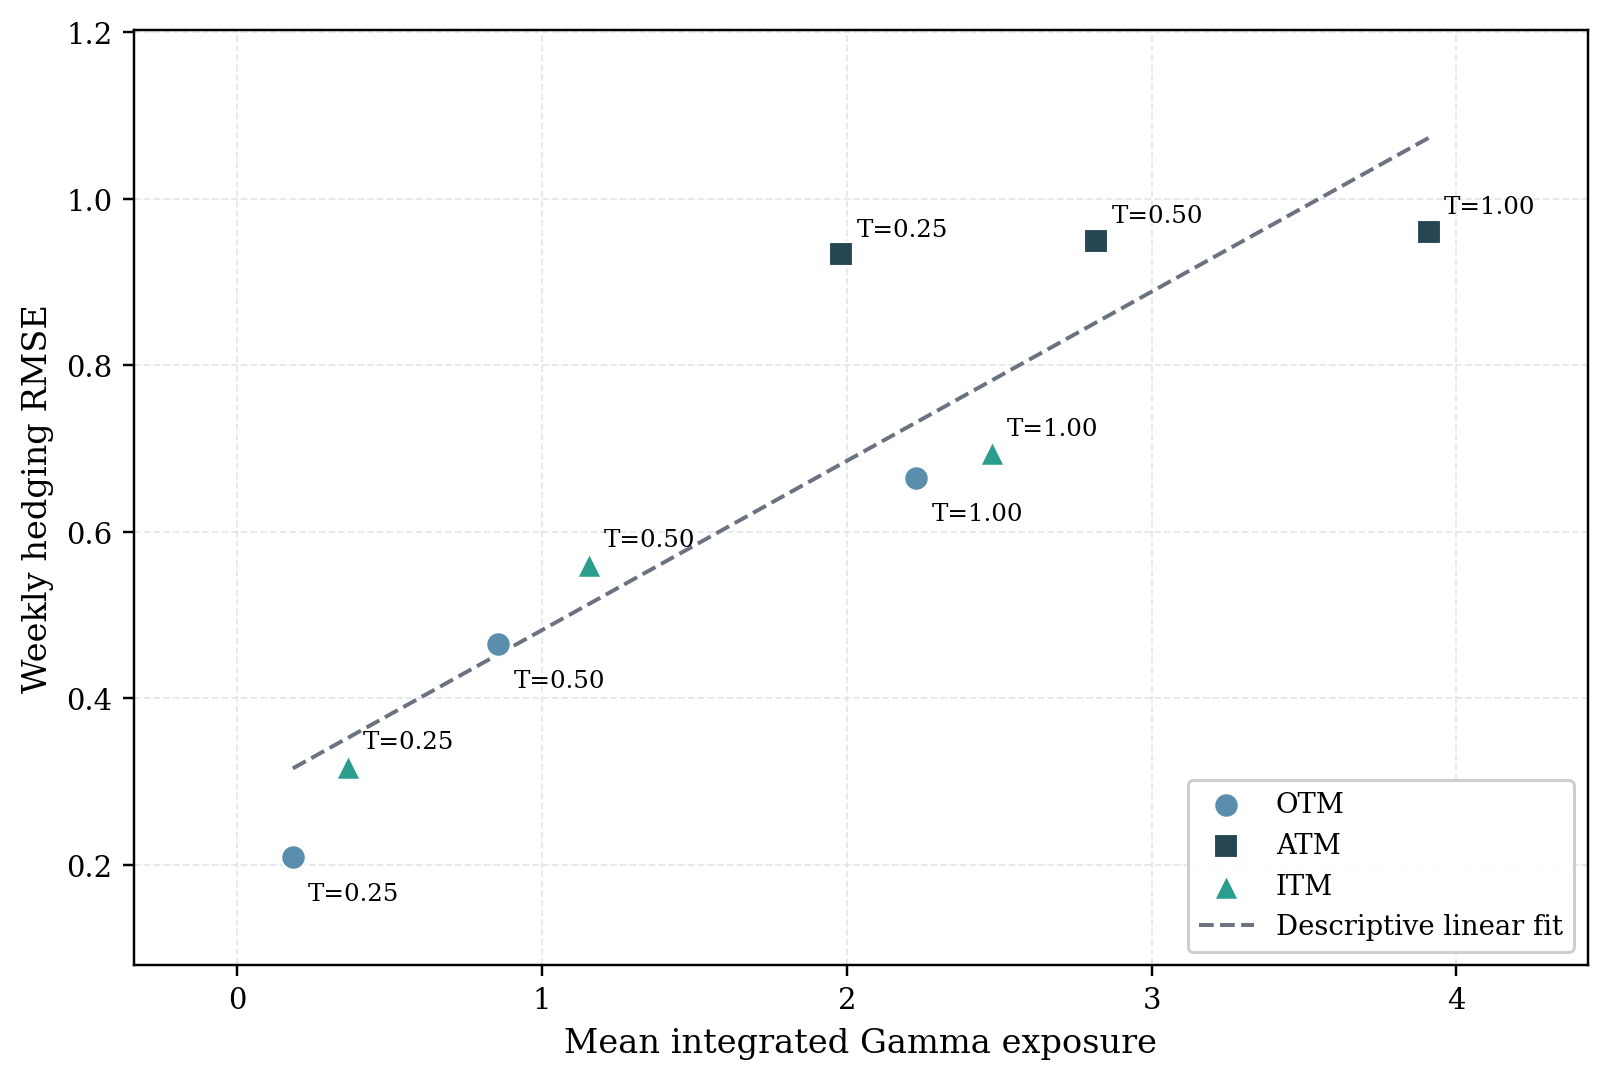
\includegraphics[width=0.55\linewidth]{gamma_exposure_rmse.png}
    \caption{Scenario-level association between mean integrated Gamma exposure and weekly hedging RMSE. The bootstrap interval is based on the nine plotted scenario pairs.}
    \label{fig:gamma_rmse}
\end{figure}

At the individual-path level, the relationship was weaker but positive: the pooled weekly Pearson correlation between pathwise Gamma exposure and absolute hedging error was approximately \WeeklyPathPearson, and the Spearman correlation was approximately \WeeklyPathSpearman. The difference between scenario- and path-level results reinforces the interpretation of $G$ as a risk indicator rather than a complete explanation of realised error.

The same nine-scenario experiment was rerun at all four hedge frequencies. Table~\ref{tab:gamma_robustness} shows that the scenario-level association remains positive under monthly, weekly, twice-weekly, and daily rebalancing, with bootstrap intervals generated from the same documented procedure.

\begin{table}[H]
\centering
\caption{Scenario-level Gamma-exposure association across hedge frequencies.}
\label{tab:gamma_robustness}
\begin{tabular}{lrrr}
\toprule
Frequency & Pearson $r$ & Spearman $\rho$ & Bootstrap 95\% CI \\
\midrule
Monthly & 0.917 & 0.950 & [0.746, 0.995] \\
Weekly & 0.903 & 0.950 & [0.709, 0.990] \\
Approx. twice-weekly & 0.897 & 0.883 & [0.693, 0.992] \\
Daily & 0.910 & 0.950 & [0.734, 0.993] \\
\bottomrule
\end{tabular}
\end{table}


These findings do not establish causality. As Equation~\eqref{eq:local_residual} indicates, realised error depends on signed squared-price innovations, timing, and the hedge grid, while the exposure proxy aggregates a non-negative Gamma-scaled variance measure. Both quantities are generated by the same paths. The evidence therefore supports a stable association between cumulative convexity exposure and hedging risk across the tested scenarios.

\FloatBarrier

\subsection{RQ4: Transaction Costs and the Accuracy--Cost Trade-off}

Introducing proportional transaction costs changed the relationship between hedge frequency and replication performance. With zero costs, daily rebalancing produced the smallest RMSE among the four schedules. Daily hedging remained the lowest-RMSE schedule at 5 and 10 basis points, but the margin over less frequent schedules narrowed as costs increased.

At the highest tested cost of 25 basis points, the ranking changed. \BestTwentyFiveFrequency{} rebalancing produced the lowest RMSE, \BestTwentyFiveRMSE{}, while daily hedging produced an RMSE of \DailyTwentyFiveRMSE{}. Figure~\ref{fig:tc_heatmap} shows the resulting interaction between cost and frequency.

\begin{figure}[H]
    \centering
    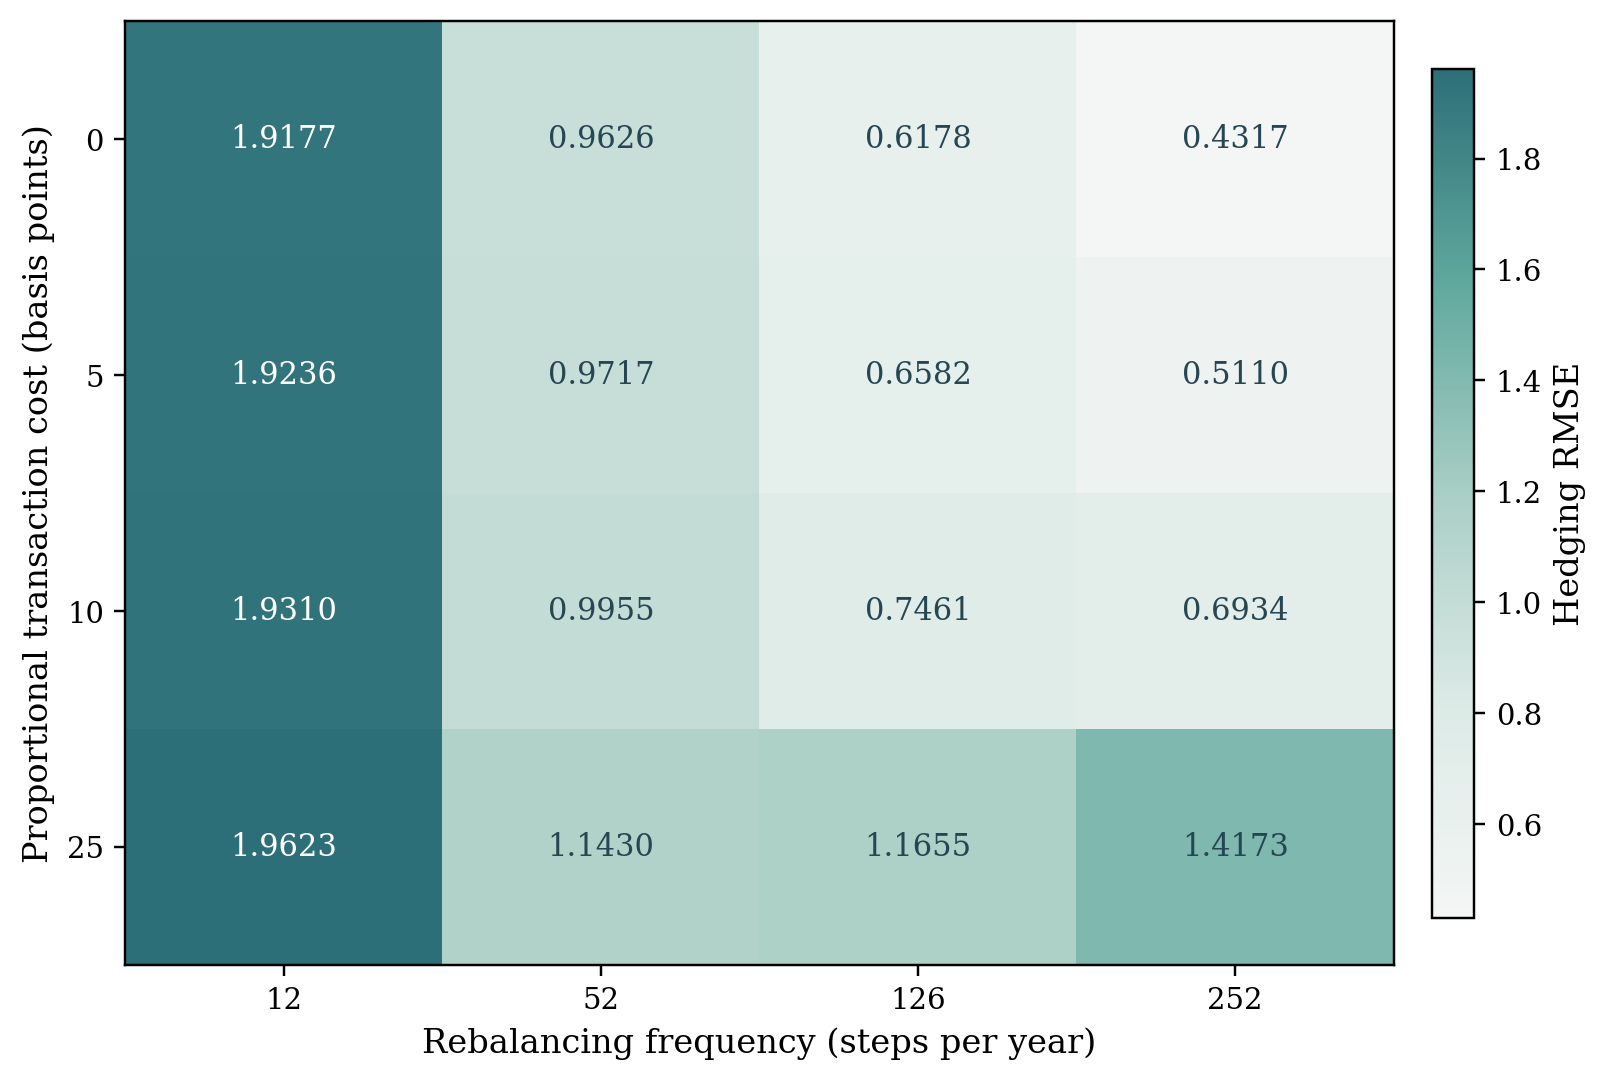
\includegraphics[width=0.8\linewidth]{transaction_cost_heatmap.png}
    \caption{Net hedging RMSE across transaction-cost levels and rebalancing frequencies. 
    Lower values indicate better replication performance.}
    \label{fig:tc_heatmap}
\end{figure}

Transaction costs also shifted mean net hedging error below zero because every hedge adjustment reduced portfolio value. Under the 10 bps assumption, for example, the mean daily hedging error was approximately $\DailyTenMeanError$, compared with a value close to zero in the frictionless experiment. The complete RMSE grid is reported in Appendix~\ref{app:tc} rather than repeated in the main text.

The results show that the frictionless benefit of more frequent rebalancing need not remain monotonic once costs become sufficiently large. Weekly rebalancing is not claimed to be universally optimal; it is merely the lowest-RMSE schedule at 25 bps within the four tested frequencies.

\section{Discussion}

The pricing results illustrate two different error mechanisms. Standard Monte Carlo error is stochastic and follows the expected square-root law. The fitted slope, its standard error, confidence interval, and $R^2$ show that the observed rate is not simply asserted from a single point estimate. The CRR error is deterministic and oscillatory. The approximately $O(N^{-1})$ even-step pattern and the odd--even effect are consistent with research showing that binomial convergence depends on payoff smoothness and strike alignment \citep{leisenreimer1996,hestonzhou2000,dienerdiener2004}. The final analysis intentionally avoids treating wall-clock timing as a reproducible model property because such measurements are environment-specific.

The sensitivity results connect static Greeks with hedge implementation. Gamma is concentrated near the strike and becomes sharper close to expiry. The second-order approximation in Section~\ref{sec:gamma_motivation} explains why this concentration is relevant: after Delta removes the first-order exposure, the leading residual contains Gamma multiplied by a centred squared-price innovation. More frequent rebalancing reduces the length of each exposure interval, which is consistent with the observed decline in frictionless RMSE.

The integrated exposure result adds a cross-scenario perspective. A high scenario-level correlation and a positive bootstrap interval indicate that scenarios with larger cumulative convexity exposure tend to have larger hedging RMSE. The weaker path-level correlations show the boundary of the result. Integrated Gamma exposure identifies where replication risk is concentrated, but it does not determine the sign or magnitude of each realised terminal error. Calling the relationship causal would ignore the common dependence of both variables on the simulated stock path.

Transaction costs reverse part of the frictionless frequency ranking. At low costs, the reduction in discretisation error dominates, so high-frequency rebalancing remains beneficial. At the highest tested cost, turnover becomes large enough to offset this benefit. This is consistent with the transaction-cost literature, in which hedging intensity is determined by a balance between risk reduction and implementation expense \citep{leland1985,toft1996,grannanswindle1996,whalleywilmott1997}. The numerical optimum is consequently conditional on the experiment rather than a general trading prescription.

Taken together, the experiments show why pricing and hedging should not be evaluated separately. Accurate valuation against an analytical benchmark does not guarantee accurate discrete replication. Likewise, a hedge schedule that performs well in a frictionless model may be unattractive once trading costs are included. The practical performance of a model depends on how its continuous-time assumptions are translated into numerical and trading decisions.

\section{Limitations}

Several limitations should be considered. First, the experiments are conducted entirely within the Black--Scholes framework. Constant volatility and interest rates are assumed, and dividends, jumps, stochastic volatility, liquidity effects, and other market imperfections are excluded. Second, the analysis uses simulated rather than observed market data; it tests internal consistency under a known data-generating process rather than forecasting or calibration performance.

Third, transaction costs are modelled as symmetric proportional charges. Bid--ask spreads, commissions, market impact, lot-size constraints, and time-varying liquidity are not represented. Fourth, the integrated Gamma-exposure measure is a theoretically motivated proxy, not an exact decomposition of terminal replication error. Each scenario-level bootstrap interval is based on only nine deliberately selected moneyness--maturity pairs, so the intervals describe sensitivity to that experimental grid rather than sampling from a broader market population. Wall-clock runtime is excluded from the final conclusions because it depends on implementation and hardware.

These restrictions are deliberate because they isolate the numerical mechanisms of interest, but they limit direct empirical application. Natural extensions include market calibration, stochastic-volatility or jump models, alternative loss functions, and adaptive or state-dependent hedging rules.

\section{Conclusion}

This study developed a unified numerical investigation of European option pricing and dynamic delta hedging within the Black--Scholes framework. By combining analytical valuation, Monte Carlo simulation, CRR binomial pricing, sensitivity analysis, discrete replication, Gamma-exposure analysis, and proportional transaction costs, it examined how theoretical pricing results are affected by numerical approximation and hedge implementation.

For RQ1, both numerical methods converged toward the analytical benchmark, but their behaviour differed. Monte Carlo produced a fitted MAE slope of $\MCSlope$ (SE $\MCSE$, 95\% CI $[\MCCILow,\MCCIHigh]$, $R^2=\MCRSquared$), consistent with $O(N^{-1/2})$. The CRR model displayed a clear odd--even oscillation, while the tested even-step sequence followed a slope of approximately $\CRRSlope$, consistent with an empirical $O(N^{-1})$ error pattern for this setup.

For RQ2, option value and the principal Greeks varied materially with the underlying price, volatility, and maturity. Gamma became increasingly concentrated near the strike as expiry approached, identifying short-dated ATM options as a region of rapid Delta variation and heightened discrete-hedging sensitivity.

For RQ3, more frequent delta rebalancing reduced terminal RMSE in the frictionless simulation. The second-order Taylor--It\^o approximation explains why local convexity is relevant once first-order Delta exposure is removed. Across the nine weekly scenarios, mean integrated Gamma exposure and hedging RMSE had a Pearson correlation of \WeeklyGammaPearson{} with a bootstrap 95\% interval of $[\WeeklyGammaCILow,\WeeklyGammaCIHigh]$. The association remained positive across all four hedge-frequency robustness runs, but weaker path-level correlations and the shared path dependence of both measures mean that Gamma exposure should be interpreted as a risk indicator, not a causal explanation.

For RQ4, proportional transaction costs weakened the frictionless benefit of frequent rebalancing. At the highest tested cost, the highest-frequency strategy no longer produced the smallest RMSE among the candidate schedules. The preferred frequency therefore depends on the cost and frequency grid rather than on a universal rule.

Overall, the study shows that pricing accuracy, local convexity, hedge frequency, and market frictions must be considered jointly. Its main contribution is an integrated and reproducible computational framework, not a new option-pricing model. Extensions to empirical market data, stochastic volatility, and adaptive hedging offer natural directions for further research.

\section*{Data and Code Availability}
All results are generated from simulated data; no proprietary or confidential market data are used. The complete source code, fixed experiment configuration, generated CSV files, statistical summaries, figure-generation scripts, LaTeX result macros, and dependency lock file are publicly available at \url{https://github.com/zhengli0426/option-pricing-delta-hedging}. Running \texttt{python -m option\_hedging reproduce --force} from the repository root regenerates the numerical evidence used by this manuscript.

\bibliographystyle{plainnat}
\bibliography{references}

\appendix

\section{Transaction-Cost Sensitivity Results}
\label{app:tc}

Table~\ref{tab:tc_appendix} reports the complete RMSE grid used in the transaction-cost sensitivity analysis.

\begin{table}[H]
\centering
\caption{Net hedging RMSE under proportional transaction costs.}
\label{tab:tc_appendix}
\begin{tabular}{lrrrr}
\toprule
Cost & Monthly & Weekly & 126/year & Daily \\
\midrule
0 bps & 1.9177 & 0.9626 & 0.6178 & 0.4317 \\
5 bps & 1.9236 & 0.9717 & 0.6582 & 0.5110 \\
10 bps & 1.9310 & 0.9955 & 0.7461 & 0.6934 \\
25 bps & 1.9623 & 1.1430 & 1.1655 & 1.4173 \\
\bottomrule
\end{tabular}
\end{table}


\section{Reproducibility Notes}
\label{app:reproducibility}

All numerical experiments were implemented in Python using standard scientific-computing libraries, including NumPy and SciPy. The Black--Scholes formulas, Monte Carlo simulation, CRR tree, Greek calculations, and discrete delta-hedging procedures were implemented directly rather than obtained from external pricing software.

The principal Monte Carlo convergence experiment used sample sizes from $10^2$ to $10^6$ with 50 independent replications at each size. The frictionless hedging experiment used 5,000 GBM paths for each of the four annualised hedge frequencies. The Gamma-exposure analysis considered nine combinations of $S_0\in\{80,100,120\}$ and $T\in\{0.25,0.50,1.00\}$ at each of the same four hedge frequencies, again using 5,000 paths per scenario.

The Monte Carlo slope uncertainty was calculated by ordinary least squares on the five pairs $(\log N,\log\operatorname{MAE}_N)$. The 95\% interval used the regression standard error with three residual degrees of freedom. For every hedge frequency, the Gamma-exposure confidence interval was produced by resampling the corresponding nine scenario pairs with replacement 200,000 times and taking the 2.5th and 97.5th percentiles of the Pearson correlation. The bootstrap seed is 20260923.

Transaction-cost experiments used rates of 0, 5, 10, and 25 basis points per dollar traded. Within each hedge frequency, the same generated stock paths were reused across cost specifications; the zero-cost slice is therefore exactly the frictionless experiment rather than a separate stochastic run. A semantic seed is deterministically derived from the master seed and experiment label, and every derived seed is exported in \texttt{seed\_manifest.csv}. Numerical outputs, statistics, figures, and LaTeX result fragments are generated by a single command from \texttt{config/study.json}. The committed \texttt{manifest.json} records SHA-256 hashes for deterministic scientific outputs; wall-clock timing is intentionally excluded.

\end{document}
